\documentclass[12pt,a4paper]{article}
\usepackage[utf8]{inputenc}
\usepackage[spanish]{babel}
\usepackage{geometry}
\usepackage{graphicx}
\usepackage{xcolor}
\usepackage{tikz}
\usepackage{fancyhdr}
\usepackage{setspace}
\usepackage{amsmath}
\usepackage{amsfonts}
\usepackage{amssymb}
\usepackage{url}
\usepackage{listings}
\usepackage{float}
\usepackage{caption}
\usepackage{subcaption}

% Configuración de márgenes
\geometry{margin=2.5cm}

% Configuración de encabezados y pies de página
\pagestyle{fancy}
\fancyhf{}
\cfoot{\thepage}

% Espaciado entre líneas
\onehalfspacing

% Definir colores personalizados
\definecolor{azulcarrera}{RGB}{52, 152, 219} % Color azul para elementos de la carrera
\definecolor{colorcarrera}{HTML}{485057} % Color gris oscuro para carrera
\definecolor{colormateria}{HTML}{C45911} % Color naranja para materia
\definecolor{colordescripcion}{HTML}{1F3864} % Color azul oscuro para descripción
\definecolor{coloralumno}{HTML}{538135} % Color verde para alumno
\definecolor{colornivel}{HTML}{485057} % Color gris oscuro para nivel

% Comando para líneas grises de separación
\newcommand{\grayline}{\noindent\textcolor{gray}{\rule{\textwidth}{1pt}}}

% Configuración para incluir imágenes
\graphicspath{{./}{./images/}} % Ruta donde buscar las imágenes

% Configuración para código
\lstset{
    basicstyle=\ttfamily\footnotesize,
    breaklines=true,
    frame=single,
    numbers=left,
    numberstyle=\tiny,
    showstringspaces=false,
    captionpos=b
}

\begin{document}

% ==================== CARÁTULA ====================
\begin{titlepage}
    \centering
    
    \vspace*{1cm}
    
    % Logo de la carrera
    
\includegraphics[height=3cm]{sw-logo.png}
    
    \vspace{1.5cm}
    
    % Nombre de la Carrera
    {\huge \color{colorcarrera} \textbf{Software}}\\[1cm]
    
    % Nombre de la Materia
    {\huge \color{colormateria} \textbf{Desarrollo de Aplicaciones Móviles}}\\[1.5cm]
    
    % Descripción del trabajo a realizar
    {\LARGE \color{colordescripcion} \textbf{Manual de Desarrollador: Sistema de Notificaciones Push en Flutter}}\\[2cm]
    
    % Nombre del alumno
    {\LARGE \color{coloralumno} \textbf{Julio Viche}}\\[1cm]
    
    % Nivel
    {\LARGE \color{colornivel} \textbf{6° Semestre}}
    
    \vspace{1cm}
    \vfill
    
    % Decoración celeste inferior
    \begin{tikzpicture}[remember picture, overlay]
        \node[anchor=south] at ([yshift=0.5cm]current page.south) 
        {
\includegraphics[width=1.1\textwidth]{decoration.png}};
    \end{tikzpicture}
    
\end{titlepage}

\newpage

% ==================== CONTENIDO DEL DOCUMENTO ====================

\section*{Actividad:}
\grayline{}
\vspace{0.3cm}

Desarrollar una aplicación móvil en Flutter que implemente un sistema completo de notificaciones push, incluyendo:

\begin{itemize}
    \item Notificaciones locales instantáneas
    \item Notificaciones con botones de acción
    \item Notificaciones programadas con temporizador
    \item Notificaciones remotas mediante Firebase Cloud Messaging
    \item Manejo de notificaciones en tres estados: Foreground, Background y Terminated
    \item Sistema de persistencia con base de datos SQLite
    \item Interfaz de usuario con navegación mediante rutas
\end{itemize}

\vspace{1cm}

\section*{Objetivo:}
\grayline{}
\vspace{0.3cm}

Comprender e implementar un sistema robusto de notificaciones push en Flutter, dominando las técnicas para manejar notificaciones locales y remotas en diferentes estados de la aplicación, incluyendo la configuración de Firebase Cloud Messaging, la programación de notificaciones con temporizador, y la implementación de una arquitectura escalable con persistencia de datos mediante SQLite.

\vspace{1cm}

\section*{Introducción:}
\grayline{}
\vspace{0.3cm}

Las notificaciones push son un componente fundamental en las aplicaciones móviles modernas, permitiendo a los desarrolladores mantener a los usuarios informados y comprometidos incluso cuando la aplicación no está activa. En el ecosistema Flutter, existen dos tipos principales de notificaciones: las \textbf{notificaciones locales}, generadas directamente desde el dispositivo del usuario, y las \textbf{notificaciones remotas}, enviadas desde un servidor externo mediante servicios como Firebase Cloud Messaging (FCM).

Este manual presenta un enfoque completo para implementar ambos tipos de notificaciones, considerando los tres estados críticos de una aplicación móvil:

\begin{itemize}
    \item \textbf{Foreground (Primer plano):} La aplicación está abierta y visible.
    \item \textbf{Background (Segundo plano):} La aplicación está ejecutándose pero minimizada.
    \item \textbf{Terminated (Cerrada):} La aplicación está completamente cerrada.
\end{itemize}

Además, se implementará un sistema de notificaciones programadas que permite a los usuarios configurar alertas para momentos específicos, con persistencia que sobrevive incluso al reinicio del dispositivo. La aplicación también incluirá una base de datos SQLite para mantener un historial completo de todas las notificaciones recibidas y generadas.

\vspace{1cm}

\section*{Desarrollo:}
\grayline{}
\vspace{0.3cm}

\subsection*{1. Configuración Inicial del Proyecto}

\subsubsection*{1.1 Dependencias Requeridas}

Para implementar el sistema de notificaciones completo, se deben agregar las siguientes dependencias en el archivo \texttt{pubspec.yaml}:

\begin{verbatim}
dependencies:
  flutter:
    sdk: flutter
  cupertino_icons: ^1.0.8
  firebase_core: ^4.2.1
  firebase_messaging: ^16.0.4
  flutter_local_notifications: ^18.0.1
  sqflite: ^2.4.1
  path_provider: ^2.1.5
  path: ^1.9.0
  intl: ^0.20.1
\end{verbatim}

\textbf{Descripción de las dependencias:}

\begin{itemize}
    \item \texttt{firebase\_core} y \texttt{firebase\_messaging}: Para notificaciones remotas mediante Firebase
    \item \texttt{flutter\_local\_notifications}: Para notificaciones locales y programadas
    \item \texttt{sqflite}: Base de datos SQLite para persistencia
    \item \texttt{path\_provider} y \texttt{path}: Manejo de rutas del sistema
    \item \texttt{intl}: Formateo de fechas y horas
\end{itemize}

\subsubsection*{1.2 Configuración de Permisos en Android}

En el archivo \texttt{android/app/src/main/AndroidManifest.xml}, se deben agregar los siguientes permisos:

\begin{verbatim}
<uses-permission android:name="android.permission.INTERNET"/>
<uses-permission android:name="android.permission.RECEIVE_BOOT_COMPLETED"/>
<uses-permission android:name="android.permission.VIBRATE"/>
<uses-permission android:name="android.permission.WAKE_LOCK"/>
<uses-permission android:name="android.permission.POST_NOTIFICATIONS"/>
<uses-permission android:name="android.permission.SCHEDULE_EXACT_ALARM"/>
<uses-permission android:name="android.permission.USE_EXACT_ALARM"/>
\end{verbatim}

Además, se deben configurar los receivers dentro del tag \texttt{<application>}:

\begin{verbatim}
<receiver 
    android:name="com.dexterous.flutterlocalnotifications.
                  ScheduledNotificationBootReceiver"
    android:exported="false">
    <intent-filter>
        <action android:name="android.intent.action.BOOT_COMPLETED"/>
    </intent-filter>
</receiver>

<receiver 
    android:name="com.dexterous.flutterlocalnotifications.
                  ActionBroadcastReceiver"
    android:exported="false"/>
\end{verbatim}

\begin{figure}[H]
    \centering
    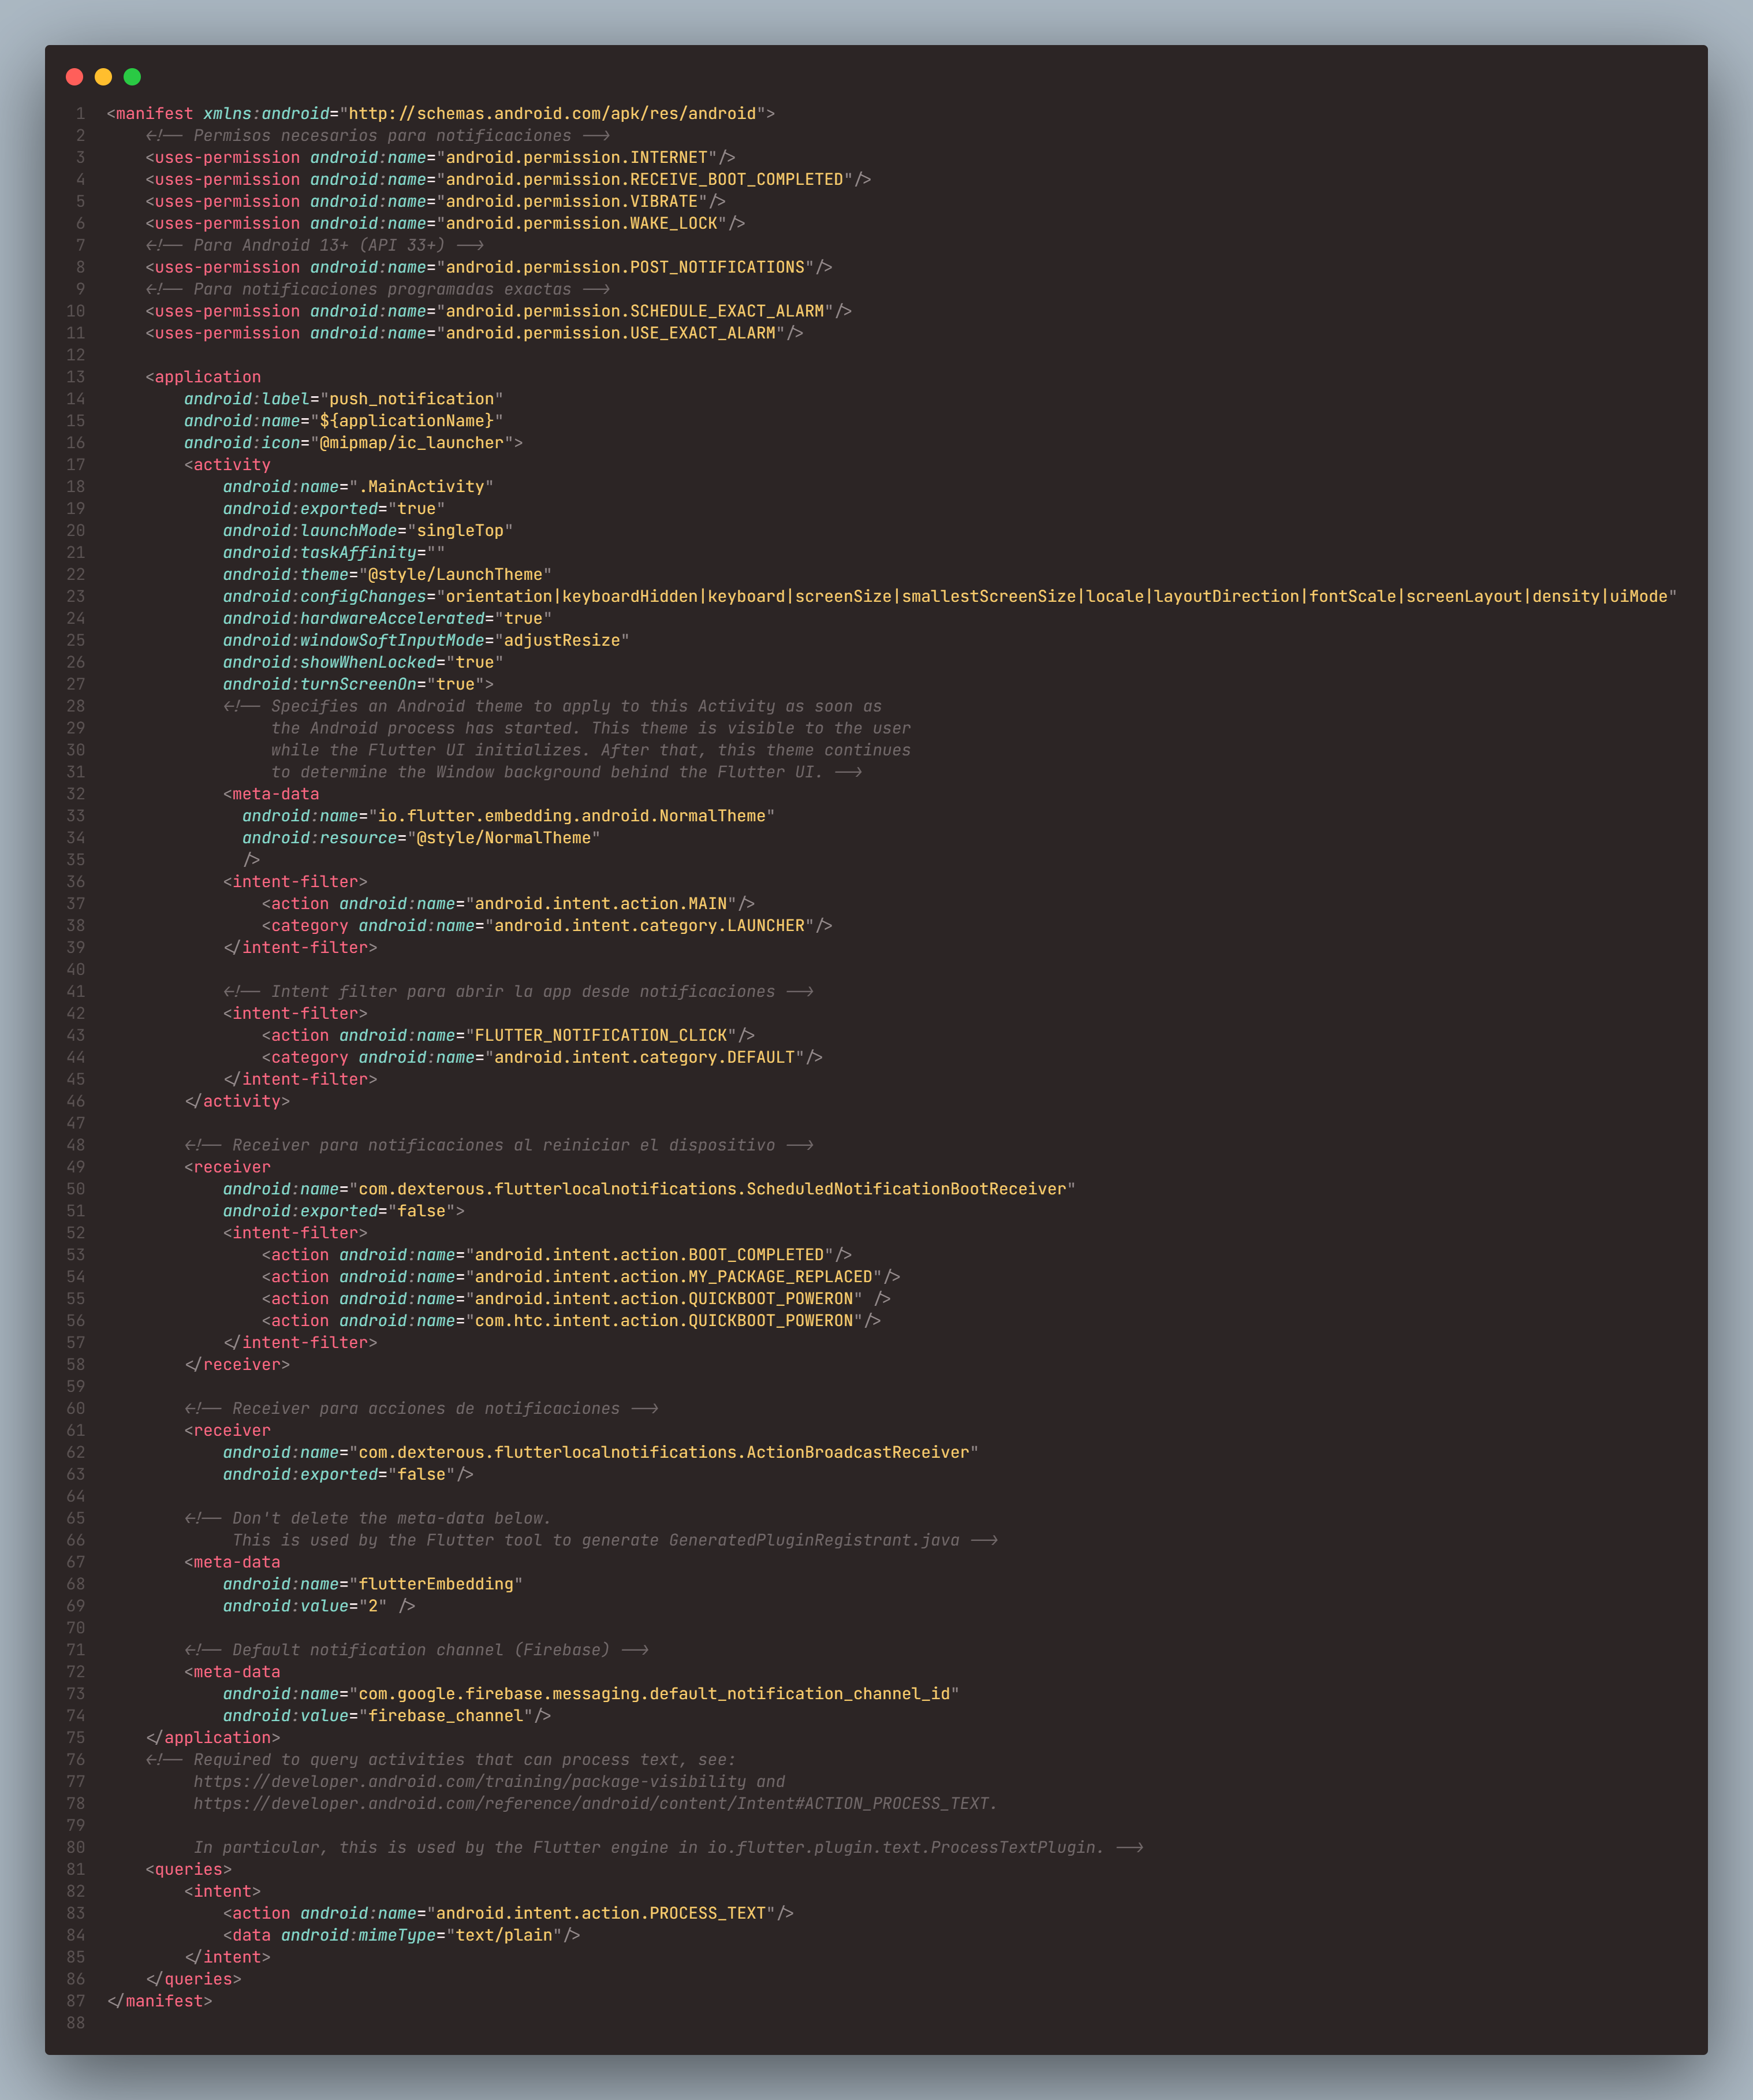
\includegraphics[width=0.9\textwidth]{androidmanifest.png}
    \caption{AndroidManifest.xml con permisos configurados}
    \label{fig:manifest}
\end{figure}

\textit{Nota: Captura del archivo AndroidManifest.xml mostrando los permisos y receivers}

\newpage

\subsection*{2. Arquitectura del Sistema}

El sistema sigue una arquitectura por capas:

\begin{verbatim}
lib/
|-- main.dart                       # Punto de entrada
|-- models/
|   +-- notification_model.dart     # Modelo de datos
|-- services/
|   |-- notification_service.dart   # Notificaciones locales
|   |-- firebase_service.dart       # Firebase Messaging
|   +-- database_service.dart       # Persistencia SQLite
|-- screens/
|   |-- home_screen.dart
|   |-- notification_list_screen.dart
|   |-- notification_detail_screen.dart
|   +-- scheduled_notification_screen.dart
+-- routes/
    +-- app_routes.dart             # Sistema de rutas
\end{verbatim}

\begin{figure}[H]
    \centering
    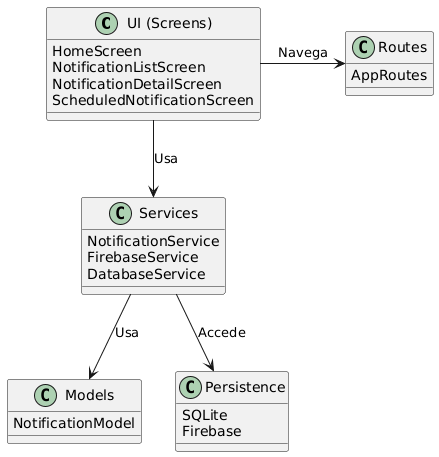
\includegraphics[width=0.8\textwidth]{arquitectura.png}
    \caption{Arquitectura del sistema de notificaciones}
    \label{fig:arquitectura}
\end{figure}

\textit{Nota: Para generar esta imagen, crear un diagrama que muestre las capas: UI (Screens) → Services → Models → Database/Firebase}

\subsection*{3. Implementación del Modelo de Datos}

El archivo \texttt{notification\_model.dart} define la estructura de datos:

\begin{verbatim}
class NotificationModel {
  final int? id;
  final String title;
  final String body;
  final DateTime timestamp;
  final String type; // 'local', 'remote', 'scheduled'
  final bool isRead;

  NotificationModel({
    this.id,
    required this.title,
    required this.body,
    required this.timestamp,
    required this.type,
    this.isRead = false,
  });

  Map<String, dynamic> toMap() {
    return {
      'id': id,
      'title': title,
      'body': body,
      'timestamp': timestamp.toIso8601String(),
      'type': type,
      'isRead': isRead ? 1 : 0,
    };
  }

  factory NotificationModel.fromMap(Map<String, dynamic> map) {
    return NotificationModel(
      id: map['id'] as int?,
      title: map['title'] as String,
      body: map['body'] as String,
      timestamp: DateTime.parse(map['timestamp'] as String),
      type: map['type'] as String,
      isRead: (map['isRead'] as int) == 1,
    );
  }
}
\end{verbatim}

\newpage

\subsection*{4. Servicio de Base de Datos (DatabaseService)}

La clase \texttt{DatabaseService} implementa el patrón Singleton y maneja todas las operaciones con SQLite:

\begin{verbatim}
class DatabaseService {
  static final DatabaseService _instance = 
      DatabaseService._internal();
  static Database? _database;

  factory DatabaseService() => _instance;
  DatabaseService._internal();

  Future<Database> get database async {
    if (_database != null) return _database!;
    _database = await _initDatabase();
    return _database!;
  }

  Future<Database> _initDatabase() async {
    String path = join(await getDatabasesPath(), 
                       'notifications.db');
    return await openDatabase(
      path,
      version: 1,
      onCreate: _onCreate,
    );
  }

  Future<void> _onCreate(Database db, int version) async {
    await db.execute('''
      CREATE TABLE notifications(
        id INTEGER PRIMARY KEY AUTOINCREMENT,
        title TEXT NOT NULL,
        body TEXT NOT NULL,
        timestamp TEXT NOT NULL,
        type TEXT NOT NULL,
        isRead INTEGER NOT NULL DEFAULT 0
      )
    ''');
  }

  Future<int> insertNotification(
      NotificationModel notification) async {
    final db = await database;
    return await db.insert('notifications', 
                           notification.toMap());
  }

  Future<List<NotificationModel>> getAllNotifications() async {
    final db = await database;
    final List<Map<String, dynamic>> maps = 
        await db.query('notifications', 
                       orderBy: 'timestamp DESC');
    return List.generate(maps.length, (i) {
      return NotificationModel.fromMap(maps[i]);
    });
  }
}
\end{verbatim}

\newpage

\subsection*{5. Servicio de Notificaciones Locales}

El \texttt{NotificationService} maneja las notificaciones locales y programadas:

\textbf{5.1 Inicialización:}

\begin{verbatim}
class NotificationService {
  final FlutterLocalNotificationsPlugin 
      _flutterLocalNotificationsPlugin =
      FlutterLocalNotificationsPlugin();

  Future<void> initialize() async {
    tz.initializeTimeZones();

    const AndroidInitializationSettings 
        initializationSettingsAndroid =
        AndroidInitializationSettings('@mipmap/ic_launcher');

    const InitializationSettings initializationSettings =
        InitializationSettings(
            android: initializationSettingsAndroid);

    await _flutterLocalNotificationsPlugin.initialize(
      initializationSettings,
      onDidReceiveNotificationResponse: _onNotificationTap,
    );

    await _requestPermissions();
  }
}
\end{verbatim}

\textbf{5.2 Notificación Instantánea:}

\begin{verbatim}
Future<void> showInstantNotification({
  required int id,
  required String title,
  required String body,
}) async {
  const AndroidNotificationDetails androidDetails =
      AndroidNotificationDetails(
    'instant_channel',
    'Notificaciones Instantáneas',
    importance: Importance.max,
    priority: Priority.high,
  );

  const NotificationDetails notificationDetails =
      NotificationDetails(android: androidDetails);

  await _flutterLocalNotificationsPlugin.show(
    id, title, body, notificationDetails,
    payload: 'instant_$id',
  );

  await _databaseService.insertNotification(
    NotificationModel(
      title: title,
      body: body,
      timestamp: DateTime.now(),
      type: 'local',
    ),
  );
}
\end{verbatim}

\newpage

\textbf{5.3 Notificación con Botones:}

\begin{verbatim}
Future<void> showNotificationWithButtons({
  required int id,
  required String title,
  required String body,
}) async {
  const AndroidNotificationDetails androidDetails =
      AndroidNotificationDetails(
    'action_channel',
    'Notificaciones con Acciones',
    importance: Importance.max,
    priority: Priority.high,
    actions: <AndroidNotificationAction>[
      AndroidNotificationAction('accept', 'Aceptar',
          showsUserInterface: true),
      AndroidNotificationAction('reject', 'Rechazar',
          cancelNotification: true),
    ],
  );

  const NotificationDetails notificationDetails =
      NotificationDetails(android: androidDetails);

  await _flutterLocalNotificationsPlugin.show(
    id, title, body, notificationDetails,
    payload: 'action_$id',
  );
}
\end{verbatim}

\textbf{5.4 Notificación Programada (Temporizador):}

\begin{verbatim}
Future<void> scheduleNotification({
  required int id,
  required String title,
  required String body,
  required DateTime scheduledDate,
}) async {
  const AndroidNotificationDetails androidDetails =
      AndroidNotificationDetails(
    'scheduled_channel',
    'Notificaciones Programadas',
    importance: Importance.max,
    priority: Priority.high,
  );

  const NotificationDetails notificationDetails =
      NotificationDetails(android: androidDetails);

  await _flutterLocalNotificationsPlugin.zonedSchedule(
    id, title, body,
    tz.TZDateTime.from(scheduledDate, tz.local),
    notificationDetails,
    androidScheduleMode: 
        AndroidScheduleMode.exactAllowWhileIdle,
    uiLocalNotificationDateInterpretation:
        UILocalNotificationDateInterpretation.absoluteTime,
  );
}
\end{verbatim}

\newpage

\subsection*{6. Servicio de Firebase Messaging}

El \texttt{FirebaseService} maneja las notificaciones remotas en los tres estados de la aplicación:

\textbf{6.1 Handler para Foreground:}

\begin{verbatim}
void _setupForegroundHandler() {
  FirebaseMessaging.onMessage.listen((RemoteMessage message) async {
    final title = message.notification?.title ?? 'Sin título';
    final body = message.notification?.body ?? 'Sin mensaje';

    await _notificationService.showFirebaseNotification(
      id: DateTime.now().millisecondsSinceEpoch ~/ 1000,
      title: title,
      body: body,
    );
  });
}
\end{verbatim}

\textbf{6.2 Handler para Background:}

\begin{verbatim}
void _setupBackgroundHandler() {
  FirebaseMessaging.onMessageOpenedApp.listen(
      (RemoteMessage message) async {
    final title = message.notification?.title ?? 'Sin título';
    final body = message.notification?.body ?? 'Sin mensaje';

    await _databaseService.insertNotification(
      NotificationModel(
        title: title,
        body: body,
        timestamp: DateTime.now(),
        type: 'remote',
      ),
    );
  });
}
\end{verbatim}

\textbf{6.3 Handler para Terminated (Función Top-Level):}

Esta función DEBE estar fuera de cualquier clase en \texttt{main.dart}:

\begin{verbatim}
@pragma('vm:entry-point')
Future<void> _firebaseBackgroundHandler(
    RemoteMessage message) async {
  await Firebase.initializeApp(
      options: DefaultFirebaseOptions.currentPlatform);
  
  final title = message.notification?.title ?? 'Sin título';
  final body = message.notification?.body ?? 'Sin mensaje';

  final databaseService = DatabaseService();
  await databaseService.insertNotification(
    NotificationModel(
      title: title,
      body: body,
      timestamp: DateTime.now(),
      type: 'remote',
    ),
  );

  final notificationService = NotificationService();
  await notificationService.initialize();
  await notificationService.showFirebaseNotification(
    id: DateTime.now().millisecondsSinceEpoch ~/ 1000,
    title: title,
    body: body,
  );
}
\end{verbatim}

Y registrarlo en el \texttt{main()}:

\begin{verbatim}
void main() async {
  WidgetsFlutterBinding.ensureInitialized();
  
  await Firebase.initializeApp(
    options: DefaultFirebaseOptions.currentPlatform,
  );
  
  // IMPORTANTE: Registrar ANTES de runApp()
  FirebaseMessaging.onBackgroundMessage(
      _firebaseBackgroundHandler);
  
  final notificationService = NotificationService();
  await notificationService.initialize();
  
  final firebaseService = FirebaseService();
  await firebaseService.initialize();
  
  runApp(const MainApp());
}
\end{verbatim}

\newpage

\subsection*{7. Implementación de Pantallas}

\textbf{7.1 Pantalla Principal (HomeScreen):}

La pantalla principal presenta cuatro botones principales:

\begin{itemize}
    \item Notificación instantánea (azul)
    \item Notificación con botones (verde)
    \item Programar notificación (naranja)
    \item Ver historial de notificaciones
\end{itemize}

También muestra el token FCM (Firebase Cloud Messaging) en la parte superior.

\begin{figure}[H]
    \centering
    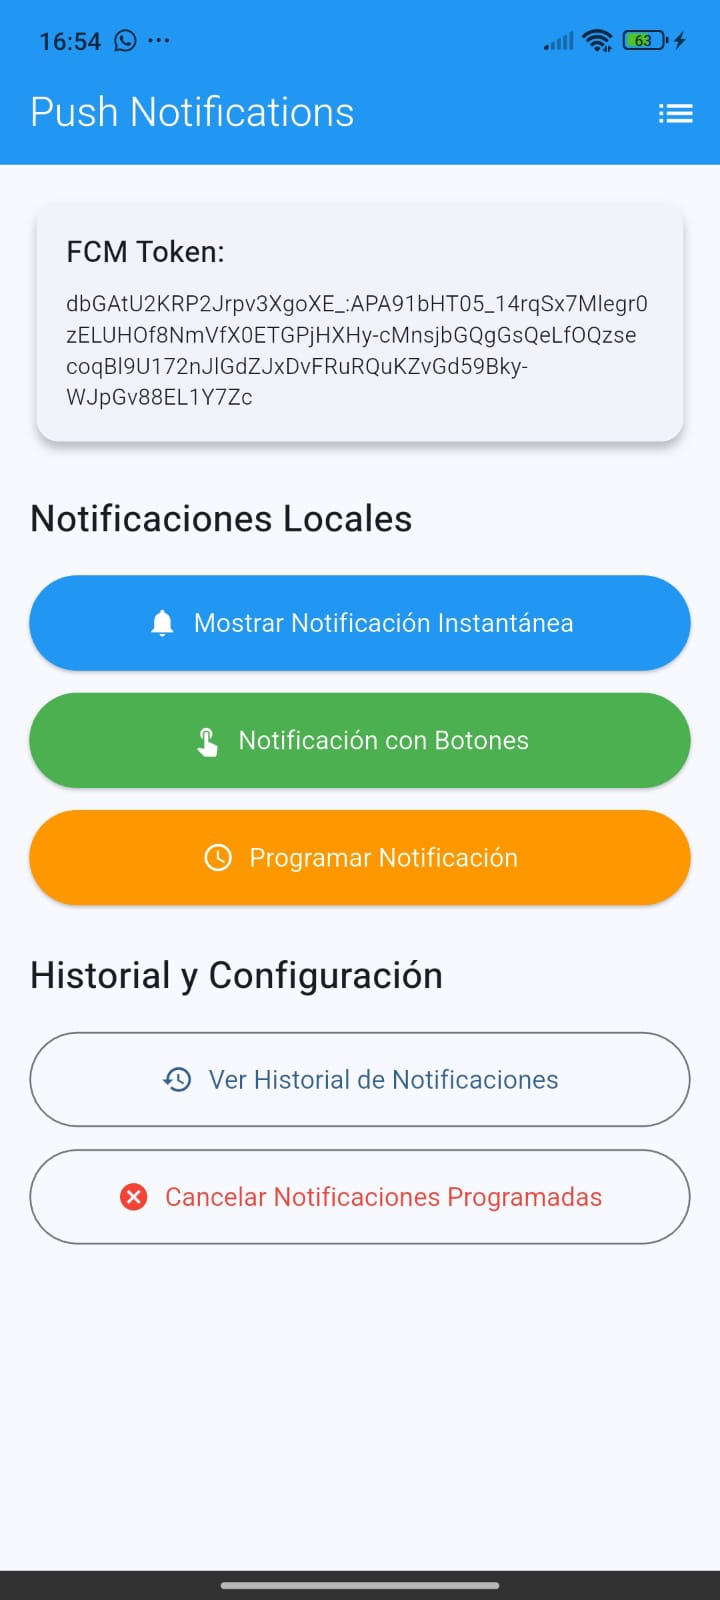
\includegraphics[width=0.5\textwidth]{home_screen.png}
    \caption{Pantalla principal de la aplicación}
    \label{fig:home}
\end{figure}

\textit{Nota: Captura de pantalla de la pantalla principal mostrando los 4 botones y el token FCM}

\vspace{0.5cm}

\textbf{7.2 Pantalla de Programación (ScheduledNotificationScreen):}

Permite al usuario:

\begin{itemize}
    \item Ingresar un título y mensaje
    \item Seleccionar fecha (desde hoy hasta 1 año adelante)
    \item Seleccionar hora exacta
    \item Ver un resumen del tiempo restante
    \item Programar la notificación
\end{itemize}

\begin{figure}[H]
    \centering
    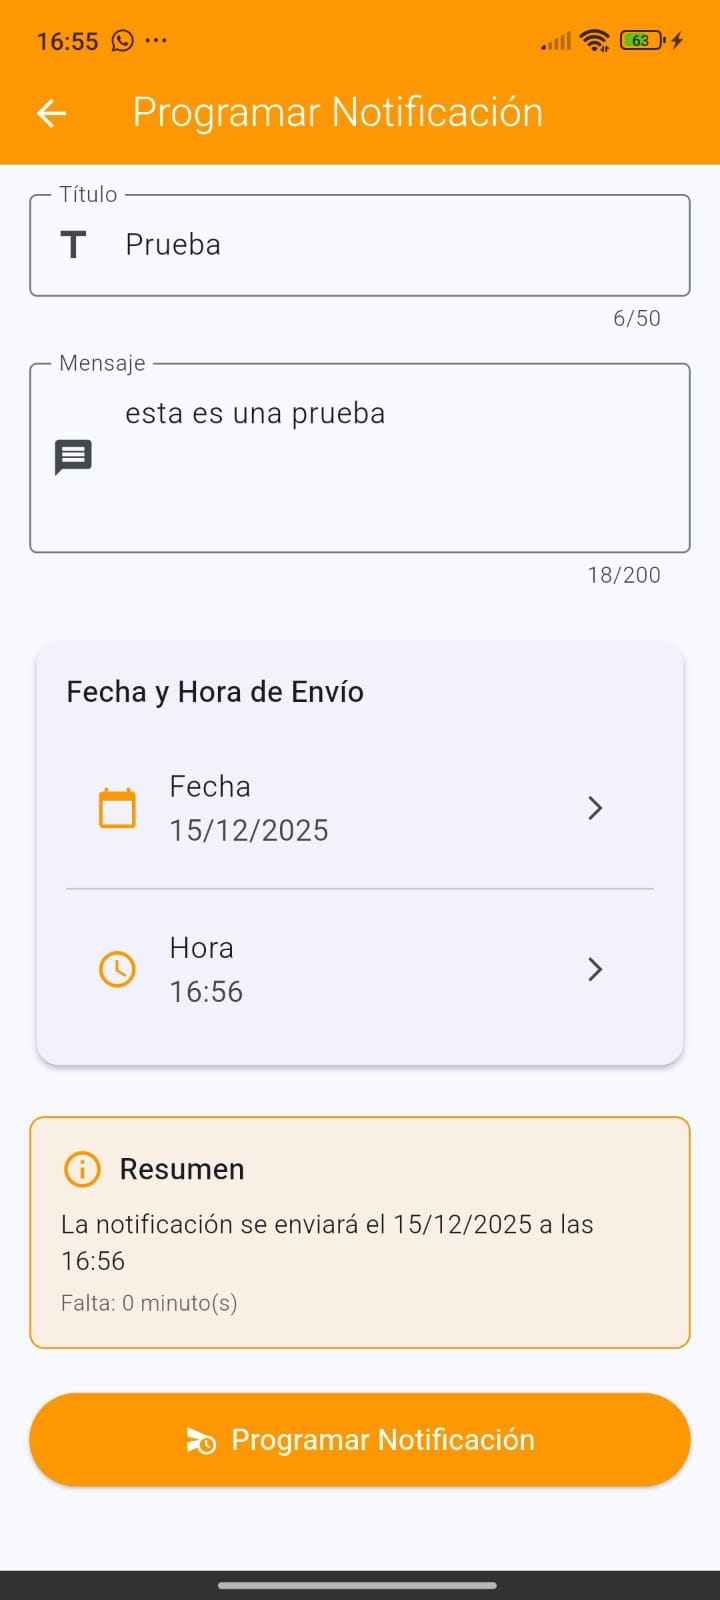
\includegraphics[width=0.5\textwidth]{schedule_screen.png}
    \caption{Pantalla de programación de notificaciones}
    \label{fig:schedule}
\end{figure}

\textit{Nota: Captura de pantalla mostrando los campos de título, mensaje, selectores de fecha/hora}

\vspace{0.5cm}

\textbf{7.3 Pantalla de Historial (NotificationListScreen):}

Muestra todas las notificaciones guardadas con:

\begin{itemize}
    \item Código de colores según tipo (local=azul, remote=verde, scheduled=naranja)
    \item Fecha y hora de cada notificación
    \item Opción de eliminar individualmente
    \item Opción de eliminar todas
    \item Pull-to-refresh para actualizar
\end{itemize}

\begin{figure}[H]
    \centering
    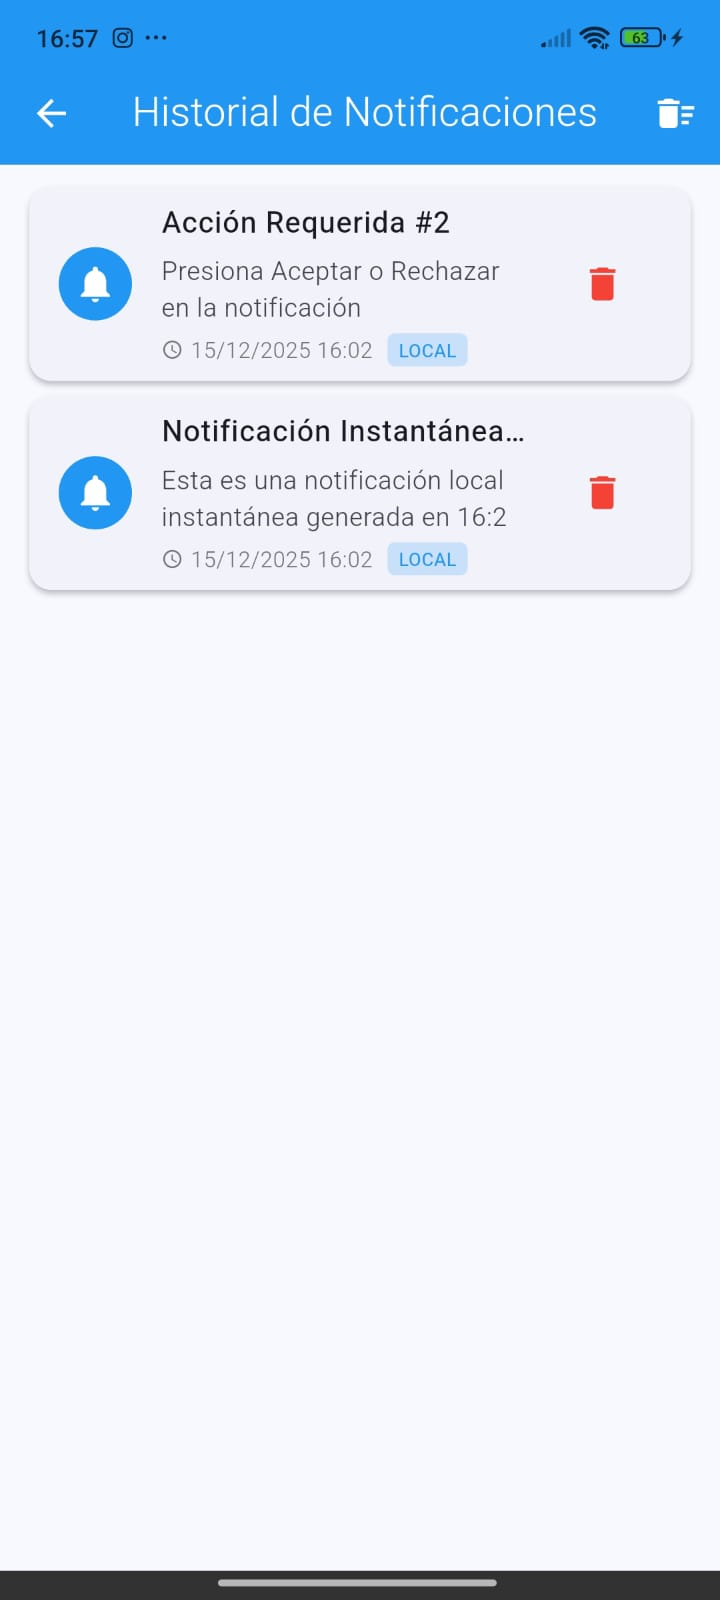
\includegraphics[width=0.5\textwidth]{notification_list.png}
    \caption{Pantalla de historial de notificaciones}
    \label{fig:list}
\end{figure}

\textit{Nota: Captura mostrando la lista de notificaciones con diferentes colores según tipo}

\vspace{0.5cm}

\textbf{7.4 Pantalla de Detalle (NotificationDetailScreen):}

Muestra información completa de una notificación:

\begin{itemize}
    \item Tipo de notificación con icono
    \item Título completo
    \item Mensaje completo
    \item Fecha y hora exacta
    \item ID de la notificación
\end{itemize}

\begin{figure}[H]
    \centering
    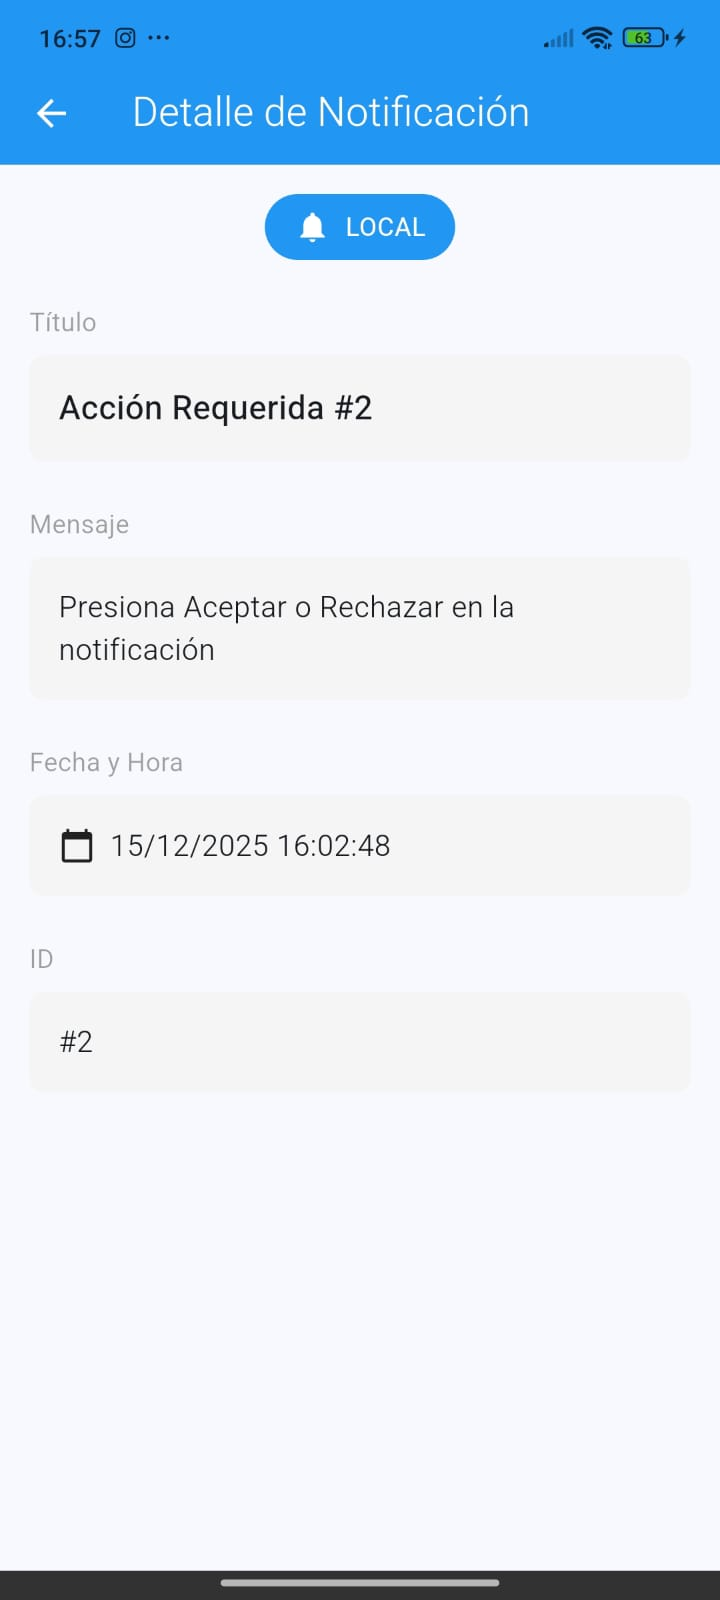
\includegraphics[width=0.5\textwidth]{notification_detail.png}
    \caption{Pantalla de detalle de notificación}
    \label{fig:detail}
\end{figure}

\textit{Nota: Captura mostrando el detalle completo de una notificación seleccionada}

\newpage

\subsection*{8. Sistema de Rutas}

El archivo \texttt{app\_routes.dart} define todas las rutas de navegación:

\begin{verbatim}
class AppRoutes {
  static const String home = '/';
  static const String notifications = '/notifications';
  static const String notificationDetail = '/notification-detail';
  static const String schedule = '/schedule';

  static Map<String, WidgetBuilder> get routes => {
    home: (context) => const HomeScreen(),
    notifications: (context) => const NotificationListScreen(),
    notificationDetail: (context) => 
        const NotificationDetailScreen(),
    schedule: (context) => 
        const ScheduledNotificationScreen(),
  };
}
\end{verbatim}

En \texttt{main.dart}, se configura el MaterialApp:

\begin{verbatim}
return MaterialApp(
  title: 'Push Notifications',
  navigatorKey: navigatorKey,
  theme: ThemeData(
    primarySwatch: Colors.blue,
    useMaterial3: true,
  ),
  initialRoute: AppRoutes.home,
  routes: AppRoutes.routes,
  onGenerateRoute: AppRoutes.onGenerateRoute,
);
\end{verbatim}

\subsection*{9. Flujos de Trabajo Completos}

\textbf{9.1 Flujo de Notificación Local Instantánea:}

\begin{enumerate}
    \item Usuario presiona botón "Mostrar Notificación Instantánea"
    \item Se llama a \texttt{NotificationService.showInstantNotification()}
    \item Se genera ID único basado en timestamp
    \item Se muestra notificación en barra de notificaciones
    \item Se guarda en base de datos SQLite
    \item Usuario hace clic en notificación
    \item App navega a pantalla de historial
\end{enumerate}

\textbf{9.2 Flujo de Notificación Programada:}

\begin{enumerate}
    \item Usuario navega a pantalla "Programar Notificación"
    \item Ingresa título y mensaje
    \item Selecciona fecha y hora deseada
    \item Presiona "Programar Notificación"
    \item Se valida que la fecha no sea pasada
    \item Se registra en el sistema operativo Android
    \item App muestra confirmación y regresa a home
    \item Al llegar la hora programada, Android dispara la notificación
    \item Notificación se muestra (incluso si app está cerrada)
    \item Al mostrarse, se guarda en base de datos
\end{enumerate}

\textbf{9.3 Flujo de Notificación Firebase (Background):}

\begin{enumerate}
    \item Servidor envía notificación mediante Firebase Console
    \item Firebase entrega mensaje al dispositivo
    \item Si app está minimizada: \texttt{onMessageOpenedApp} se activa
    \item Si app está cerrada: \texttt{\_firebaseBackgroundHandler} se ejecuta
    \item Notificación se guarda en base de datos
    \item Se muestra notificación local para consistencia
    \item Usuario hace clic en notificación
    \item App abre y navega automáticamente a historial
\end{enumerate}

\textbf{9.4 Flujo de Notificación Firebase (Terminated):}

\begin{enumerate}
    \item App está completamente cerrada
    \item Servidor envía notificación mediante Firebase
    \item Android recibe mensaje y ejecuta \texttt{\_firebaseBackgroundHandler}
    \item Handler guarda en base de datos
    \item Handler muestra notificación local
    \item Usuario hace clic en notificación
    \item Android inicia la aplicación
    \item \texttt{getInitialMessage()} recupera datos del mensaje
    \item App navega automáticamente a historial después de iniciar
\end{enumerate}

\newpage

\subsection*{10. Pruebas y Validación}

\textbf{10.1 Probar Notificaciones Locales:}

\begin{enumerate}
    \item Ejecutar la aplicación: \texttt{flutter run}
    \item Presionar botón azul "Notificación Instantánea"
    \item Verificar que aparece en barra de notificaciones
    \item Presionar botón verde "Notificación con Botones"
    \item Verificar que aparecen botones "Aceptar" y "Rechazar"
    \item Ir a "Ver Historial" y verificar que se guardaron
\end{enumerate}

\begin{figure}[H]
    \centering
    \begin{subfigure}[b]{0.45\textwidth}
        \centering
        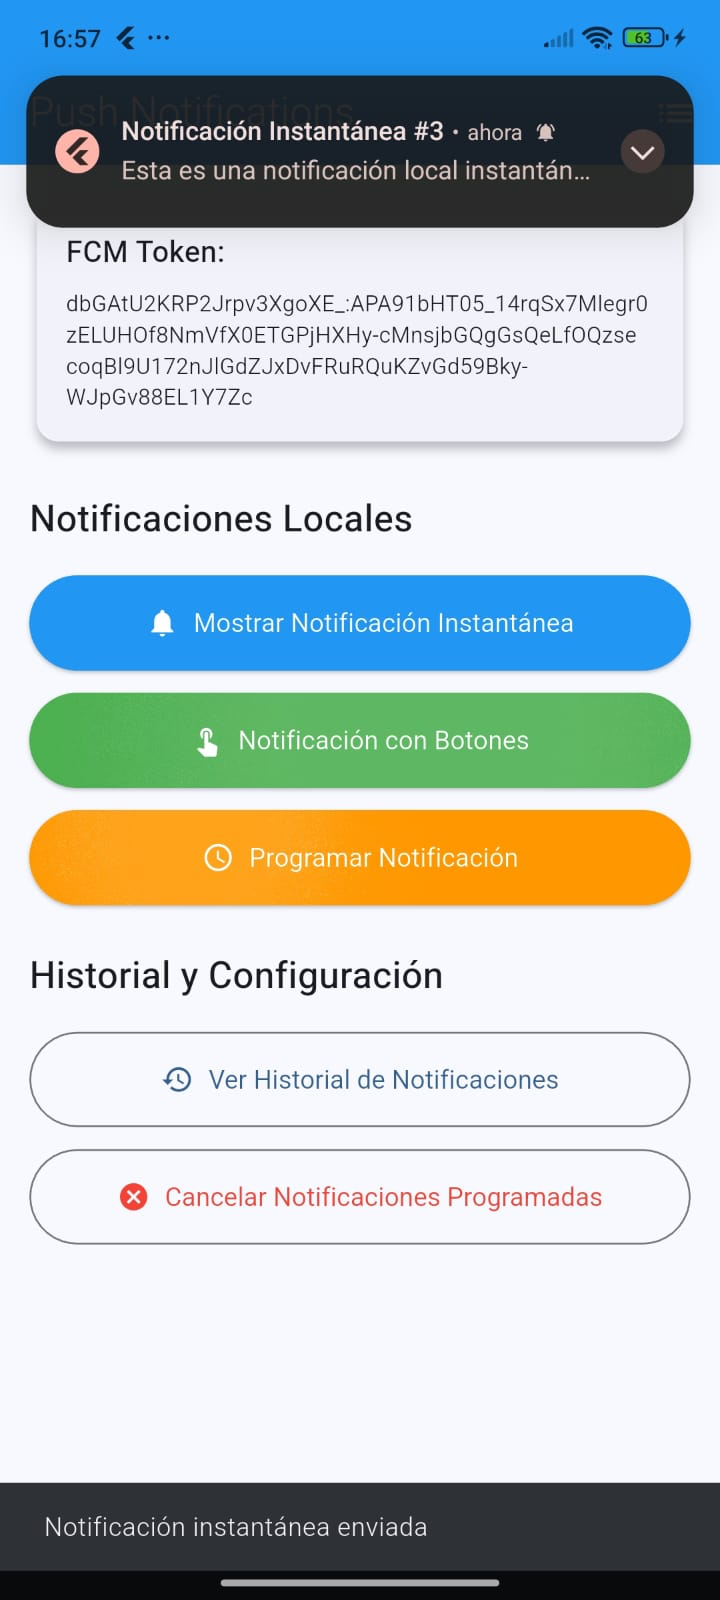
\includegraphics[width=\textwidth]{notification_instant.png}
        \caption{Notificación instantánea}
    \end{subfigure}
    \hfill
    \begin{subfigure}[b]{0.45\textwidth}
        \centering
        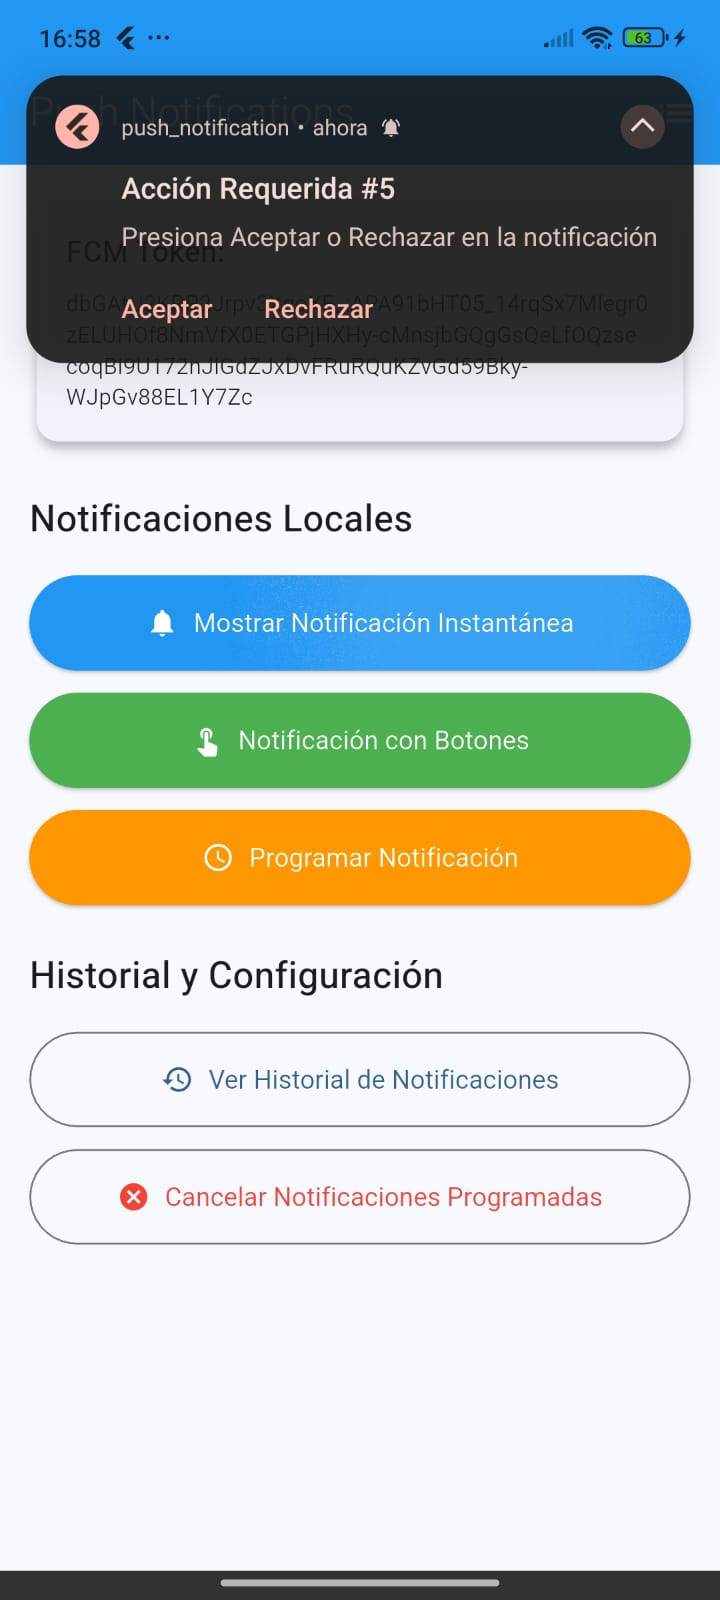
\includegraphics[width=\textwidth]{notification_buttons.png}
        \caption{Notificación con botones}
    \end{subfigure}
    \caption{Notificaciones locales en la barra de notificaciones}
    \label{fig:local_notifications}
\end{figure}

\textit{Nota: Capturas mostrando las notificaciones en la barra de notificaciones del dispositivo}

\vspace{0.5cm}

\textbf{10.2 Probar Notificación Programada:}

\begin{enumerate}
    \item Presionar botón naranja "Programar Notificación"
    \item Ingresar título: "Prueba Temporizador"
    \item Ingresar mensaje: "Esta es una notificación programada"
    \item Seleccionar fecha: Hoy
    \item Seleccionar hora: 2 minutos en el futuro
    \item Presionar "Programar Notificación"
    \item CERRAR completamente la app (swipe en recientes)
    \item Esperar los 2 minutos
    \item Verificar que la notificación aparece
    \item Hacer clic en notificación
    \item Verificar que app abre y muestra historial
\end{enumerate}

\begin{figure}[H]
    \centering
    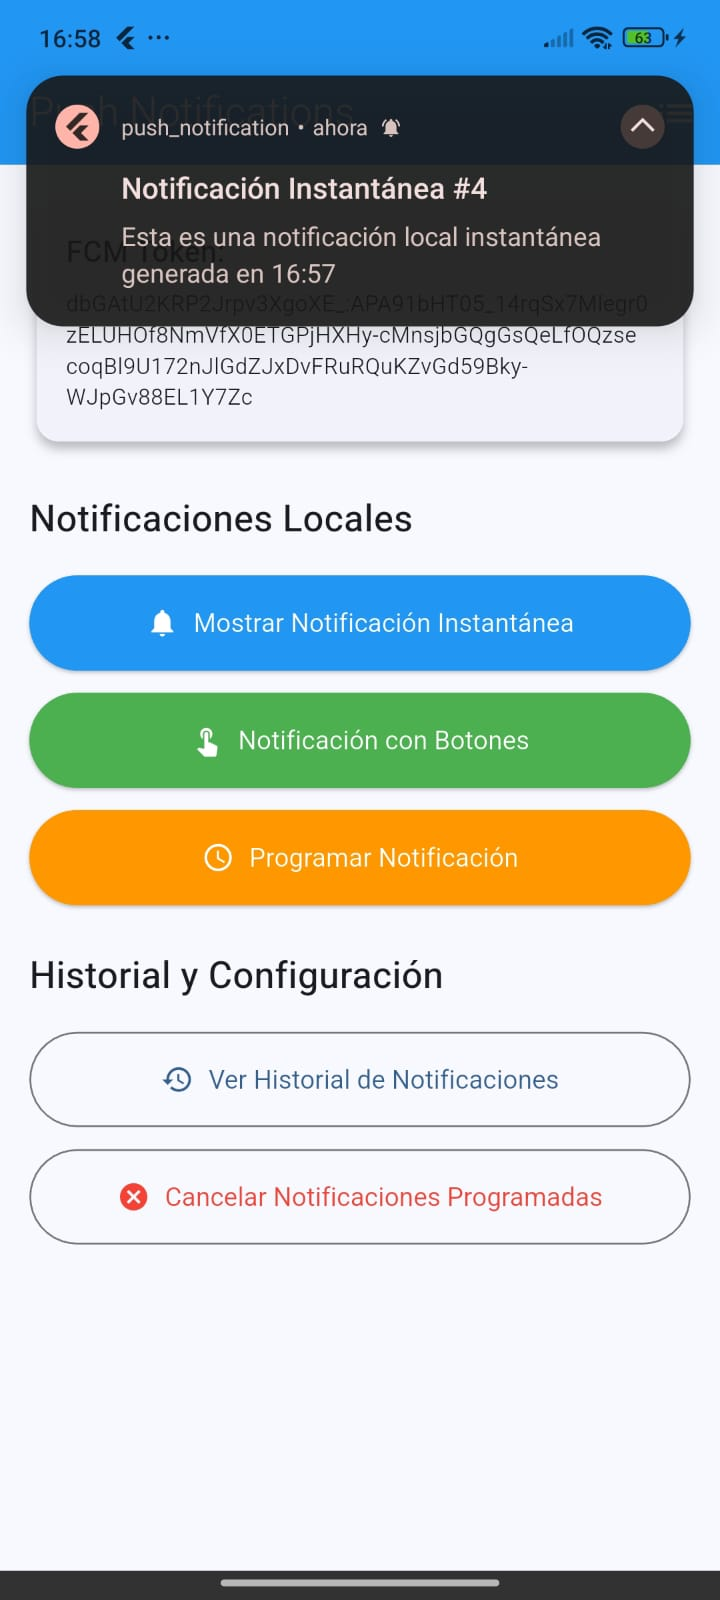
\includegraphics[width=0.5\textwidth]{notification_scheduled.png}
    \caption{Notificación programada llegando con app cerrada}
    \label{fig:scheduled}
\end{figure}

\textit{Nota: Captura mostrando la notificación programada que llegó con la app cerrada}

\vspace{0.5cm}

\textbf{10.3 Probar Notificaciones Firebase:}

\textbf{A. Foreground (App Abierta):}
\begin{enumerate}
    \item Mantener app abierta en pantalla principal
    \item Copiar el Token FCM mostrado
    \item Ir a Firebase Console → Cloud Messaging
    \item Crear nueva campaña de mensajes
    \item Título: "Prueba Foreground"
    \item Texto: "App está abierta"
    \item En "Target" pegar el token FCM copiado
    \item Enviar ahora
    \item Verificar que notificación aparece inmediatamente
    \item Verificar que se guarda en historial
\end{enumerate}

\begin{figure}[H]
    \centering
    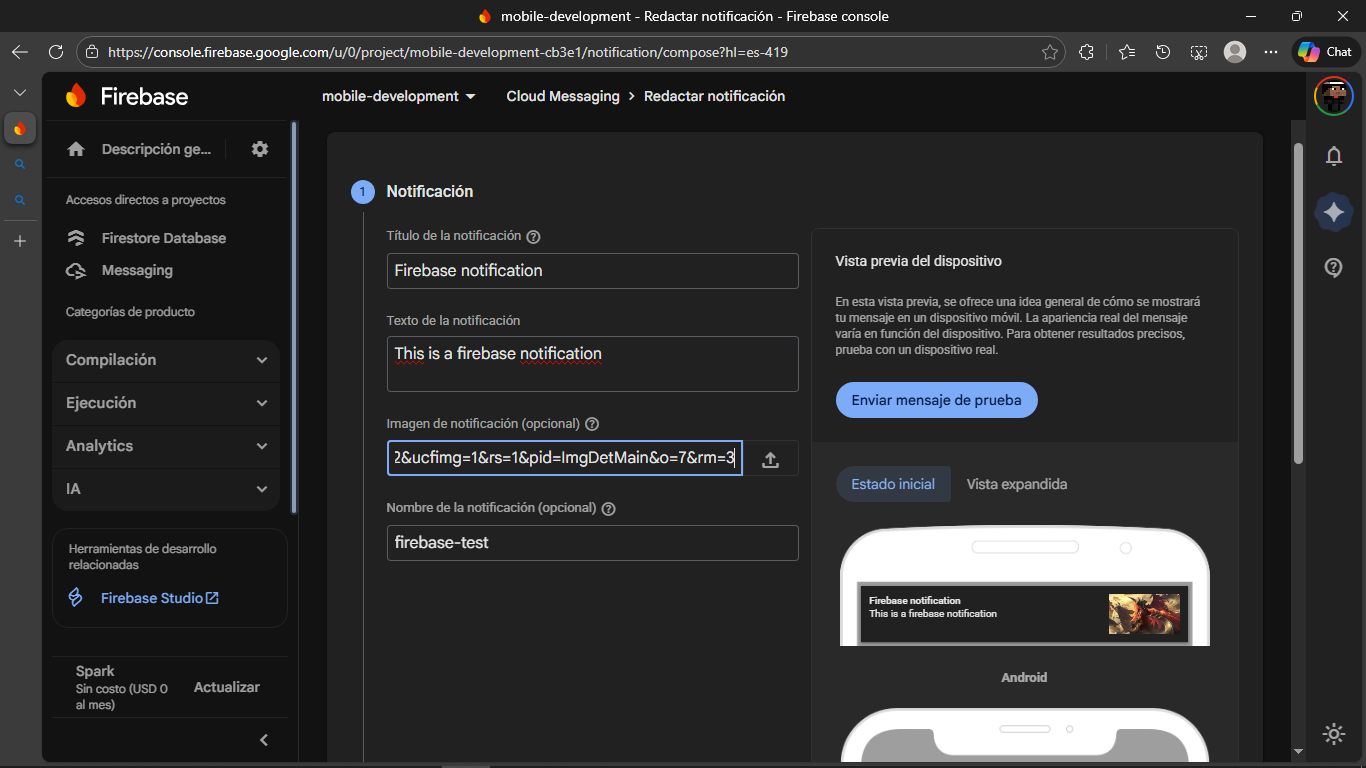
\includegraphics[width=0.8\textwidth]{firebase_console.png}
    \caption{Firebase Console - Envío de notificación}
    \label{fig:firebase_console}
\end{figure}

\textit{Nota: Captura de Firebase Console mostrando el formulario de envío de notificaciones}

\vspace{0.5cm}

\textbf{B. Background (App Minimizada):}
\begin{enumerate}
    \item Minimizar la aplicación (botón Home)
    \item Desde Firebase Console enviar notificación
    \item Título: "Prueba Background"
    \item Texto: "App en segundo plano"
    \item Verificar que aparece en barra de notificaciones
    \item Hacer clic en notificación
    \item Verificar que app abre y muestra historial
\end{enumerate}

\begin{figure}[H]
    \centering
    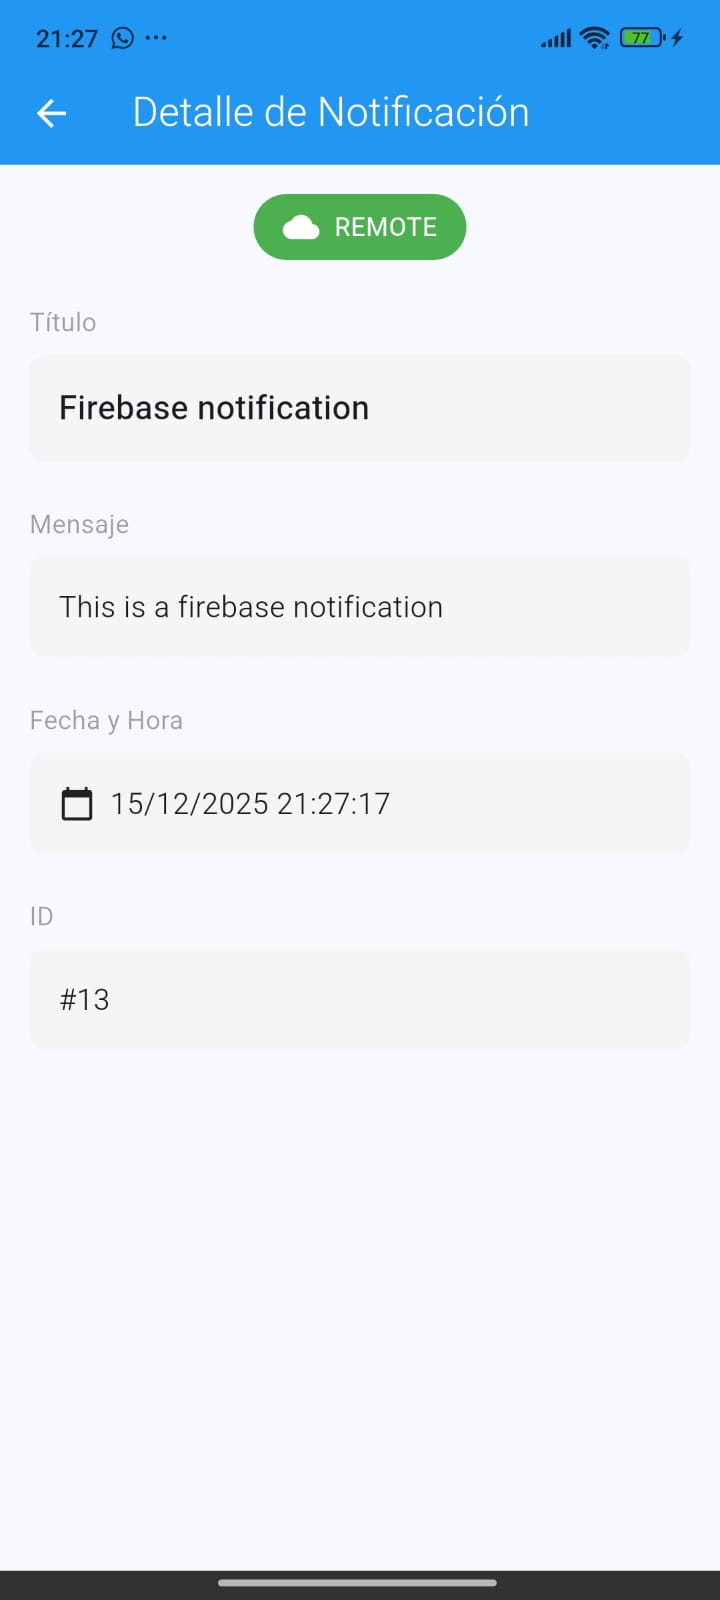
\includegraphics[width=0.5\textwidth]{notification_background.png}
    \caption{Notificación Firebase en modo Background}
    \label{fig:background}
\end{figure}

\textit{Nota: Captura de notificación Firebase recibida con app minimizada}

\vspace{0.5cm}

\textbf{C. Terminated (App Cerrada):}
\begin{enumerate}
    \item Cerrar completamente la app (swipe en recientes)
    \item Verificar que no esté en procesos activos
    \item Desde Firebase Console enviar notificación
    \item Título: "Prueba Terminated"
    \item Texto: "App estaba cerrada"
    \item Verificar que aparece en barra de notificaciones
    \item Hacer clic en notificación
    \item Verificar que app inicia desde cero
    \item Verificar que navega automáticamente a historial
    \item Verificar que la notificación está guardada
\end{enumerate}

\newpage

\subsection*{11. Solución de Problemas Comunes}

\textbf{Problema 1: Notificaciones no aparecen}

\textbf{Solución:}
\begin{itemize}
    \item Verificar permisos en Configuración → Apps → push\_notification
    \item Habilitar "Notificaciones"
    \item Para Android 13+: Aceptar permiso POST\_NOTIFICATIONS
\end{itemize}

\textbf{Problema 2: Notificaciones programadas no son exactas}

\textbf{Solución:}
\begin{itemize}
    \item Ir a Configuración → Apps → push\_notification
    \item Buscar "Alarmas y recordatorios"
    \item Habilitar permiso SCHEDULE\_EXACT\_ALARM
    \item Desactivar "Optimización de batería" para la app
\end{itemize}

\textbf{Problema 3: Firebase no entrega notificaciones}

\textbf{Solución:}
\begin{itemize}
    \item Verificar que \texttt{google-services.json} esté en \texttt{android/app/}
    \item Verificar conexión a Internet
    \item Verificar que Firebase esté inicializado correctamente
    \item Ejecutar: \texttt{flutter clean \&\& flutter pub get}
    \item Reconstruir la app: \texttt{flutter run}
\end{itemize}

\textbf{Problema 4: App no abre desde notificación}

\textbf{Solución:}
\begin{itemize}
    \item Verificar que AndroidManifest tenga \texttt{launchMode="singleTop"}
    \item Verificar que los intent-filters estén correctos
    \item Verificar que el callback \texttt{onDidReceiveNotificationResponse} esté registrado
\end{itemize}

\textbf{Problema 5: Base de datos no guarda notificaciones}

\textbf{Solución:}
\begin{itemize}
    \item Verificar que DatabaseService esté inicializado
    \item Verificar permisos de escritura en el dispositivo
    \item Limpiar datos de la app y reinstalar
    \item Verificar logs con: \texttt{flutter logs}
\end{itemize}

\newpage

\subsection*{12. Configuración de Firebase Cloud Messaging}

\textbf{Paso 1: Crear proyecto en Firebase Console}
\begin{enumerate}
    \item Ir a \url{https://console.firebase.google.com}
    \item Hacer clic en "Agregar proyecto"
    \item Ingresar nombre del proyecto
    \item Aceptar términos y crear
\end{enumerate}

\textbf{Paso 2: Agregar aplicación Android}
\begin{enumerate}
    \item En la consola de Firebase, seleccionar el proyecto
    \item Hacer clic en el ícono de Android
    \item Ingresar el package name (encontrado en \texttt{android/app/build.gradle.kts})
    \item Registrar la aplicación
    \item Descargar el archivo \texttt{google-services.json}
    \item Colocar el archivo en \texttt{android/app/}
\end{enumerate}

\textbf{Paso 3: Configurar build.gradle}

En \texttt{android/build.gradle.kts} agregar:
\begin{verbatim}
buildscript {
    dependencies {
        classpath("com.google.gms:google-services:4.4.0")
    }
}
\end{verbatim}

En \texttt{android/app/build.gradle.kts} agregar al final:
\begin{verbatim}
plugins {
    id("com.google.gms.google-services")
}
\end{verbatim}

\textbf{Paso 4: Inicializar Firebase en Flutter}

Ejecutar en terminal:
\begin{verbatim}
flutter pub add firebase_core
flutter pub add firebase_messaging
flutterfire configure
\end{verbatim}

Esto generará automáticamente el archivo \texttt{firebase\_options.dart}.

\subsection*{13. Video de Demostración}

\textbf{Link al video demostrativo (2-3 minutos):}

\vspace{0.5cm}

\textcolor{blue}{\textbf{[INSERTAR LINK DEL VIDEO AQUÍ]}}

\vspace{0.5cm}

El video muestra:
\begin{itemize}
    \item Funcionamiento completo de la aplicación
    \item Demostración de notificaciones instantáneas
    \item Demostración de notificaciones con botones
    \item Programación de notificación con temporizador
    \item Visualización del historial
    \item Prueba de notificaciones en modo Background
    \item Prueba de notificaciones en modo Terminated
    \item Código fuente de componentes principales
\end{itemize}

\textbf{Nota:} El video debe estar subido a la cuenta institucional de Google Drive o YouTube con permisos públicos de visualización.

\vspace{1cm}

\section*{Conclusiones y Recomendaciones:}
\grayline{}
\vspace{0.3cm}

\subsection*{Conclusiones}

\begin{enumerate}
    \item La implementación de un sistema completo de notificaciones push en Flutter requiere la combinación de múltiples paquetes y servicios. Firebase Cloud Messaging es esencial para notificaciones remotas, mientras que \texttt{flutter\_local\_notifications} es indispensable para notificaciones locales y programadas.

    \item El manejo de notificaciones en los tres estados de la aplicación (Foreground, Background, Terminated) presenta desafíos específicos, siendo el estado Terminated el más complejo, ya que requiere una función top-level con la anotación \texttt{@pragma('vm:entry-point')} para garantizar su correcta ejecución.

    \item La persistencia de datos mediante SQLite permite mantener un historial completo de notificaciones, mejorando significativamente la experiencia del usuario al poder consultar notificaciones pasadas en cualquier momento.

    \item La arquitectura por capas (Models, Services, Screens, Routes) facilita el mantenimiento, escalabilidad y testeo de la aplicación, separando claramente las responsabilidades de cada componente.

    \item La configuración correcta de permisos en Android, especialmente para Android 13+ (POST\_NOTIFICATIONS y SCHEDULE\_EXACT\_ALARM), es crítica para el funcionamiento del sistema de notificaciones.

    \item El uso de notificaciones programadas con \texttt{zonedSchedule} y el modo \texttt{exactAllowWhileIdle} garantiza que las notificaciones se entreguen en el momento exacto, incluso si el dispositivo se reinicia.
\end{enumerate}

\subsection*{Recomendaciones}

\begin{enumerate}
    \item \textbf{Optimización de Base de Datos:} Implementar un sistema de limpieza automática de notificaciones antiguas (por ejemplo, mayores a 30 días) para evitar que la base de datos crezca indefinidamente.

    \item \textbf{Manejo de Errores:} Implementar un sistema robusto de manejo de errores con logs detallados, especialmente para casos donde las notificaciones no se entregan por restricciones del sistema operativo.

    \item \textbf{Testing:} Realizar pruebas exhaustivas en dispositivos reales con diferentes versiones de Android (especialmente 12, 13 y 14) ya que el comportamiento de notificaciones varía significativamente entre versiones.

    \item \textbf{Optimización de Batería:} Informar al usuario sobre la necesidad de desactivar la optimización de batería para la app si requiere notificaciones programadas precisas.

    \item \textbf{UX Mejorada:} Implementar indicadores visuales más claros para notificaciones no leídas, badges en el ícono de la app y sonidos/vibraciones personalizadas según el tipo de notificación.

    \item \textbf{Seguridad:} En producción, implementar autenticación y autorización adecuadas para el sistema de notificaciones, especialmente si se integran APIs externas.

    \item \textbf{Analytics:} Integrar Firebase Analytics para rastrear métricas como tasa de apertura de notificaciones, tiempo de respuesta y engagement del usuario.

    \item \textbf{Internacionalización:} Preparar la aplicación para soporte multi-idioma desde el inicio, utilizando el paquete \texttt{flutter\_localizations}.

    \item \textbf{Documentación del Código:} Mantener comentarios claros y actualizados, especialmente en funciones críticas como los handlers de background.

    \item \textbf{CI/CD:} Implementar pipelines de integración y despliegue continuo para automatizar pruebas y distribución de la aplicación.
\end{enumerate}

\vspace{1cm}

\section*{Bibliografía (APA7):}
\grayline{}
\vspace{0.3cm}

Flutter. (2024). \textit{Flutter Local Notifications Plugin}. Recuperado de \url{https://pub.dev/packages/flutter_local_notifications}

\vspace{0.3cm}

Firebase. (2024). \textit{Firebase Cloud Messaging for Flutter}. Google. Recuperado de \url{https://firebase.google.com/docs/cloud-messaging/flutter/client}

\vspace{0.3cm}

Flutter. (2024). \textit{Firebase Messaging Plugin}. Recuperado de \url{https://pub.dev/packages/firebase_messaging}

\vspace{0.3cm}

Flutter. (2024). \textit{Sqflite - SQLite Plugin for Flutter}. Recuperado de \url{https://pub.dev/packages/sqflite}

\vspace{0.3cm}

Android Developers. (2024). \textit{Notifications Overview}. Google. Recuperado de \url{https://developer.android.com/develop/ui/views/notifications}

\vspace{0.3cm}

Android Developers. (2024). \textit{Schedule Exact Alarms}. Google. Recuperado de \url{https://developer.android.com/develop/background-work/services/alarms/schedule}

\vspace{0.3cm}

Flutter. (2024). \textit{Navigation and Routing}. Flutter Documentation. Recuperado de \url{https://docs.flutter.dev/ui/navigation}

\vspace{0.3cm}

Windmill, E. (2023). \textit{Flutter in Action}. Manning Publications.

\vspace{0.3cm}

Moroney, L. (2021). \textit{Programming Flutter: Native, Cross-Platform Apps the Easy Way}. O'Reilly Media.

\vspace{0.3cm}

Firebase. (2024). \textit{Get Started with Firebase Cloud Messaging}. Google. Recuperado de \url{https://firebase.google.com/docs/cloud-messaging/flutter/first-message}

\end{document}